\chapter{Τοπολογία Συστήματος}
\label{ch:System Topology}
Η δημιουργία φορητού (portable) λογισμικού, δηλαδή λογισμικού το οποίο μπορεί να χρησιμοποιηθεί σε συστήματα διαφορετικά μεταξύ τους, είναι δυνατή με τη χρήση αφαιρέσεων (abstractions) για το υποκείμενο σύστημα. Οι αφαιρέσεις αυτές αποκρύπτουν λεπτομέρειες της οργάνωσης του υλικού του εκάστοτε συστήματος, με την έννοια ότι από τη σκοπιά του προγραμματιστή δεν θα πρέπει να μας ενδιαφέρουν ζητήματα χαμηλού επιπέδου, όπως για παράδειγμα η οργάνωση της μνήμης από φυσική άποψη (κοινόχρηστη ή κατανεμημένη) που αναφέραμε στην Υποενότητα \ref{ssec:Classification based on memory organization}, αλλά το τι εικόνα έχουμε για αυτή.

Η αφαιρετική όμως εικόνα που έχει ο προγραμματιστής για το σύστημα που καλείται να προγραμματίσει δεν του επιτρέπει να εκμεταλλευτεί στο μέγιστο τις δυνατότητές του και άρα να επιτύχει την καλύτερη δυνατή επίδοση. Για παράδειγμα, σε ένα σύστημα δύο κόμβων με κατανεμημένη φυσική οργάνωση μνήμης που όμως παρέχει κοινόχρηστο χώρο διευθύνσεων, ναι μεν ο ένας κόμβος μπορεί να προσβεί οποιαδήποτε θέση μνήμης στον άλλο κόμβο, παρόλα αυτά το κόστος της απομακρυσμένης πρόσβασης θα είναι πολύ μεγαλύτερο από αυτό της πρόσβασης στην τοπική μνήμη.

Στον προγραμματισμό παράλληλων συστημάτων που στόχος μας είναι η επίτευξη όσο το δυνατόν καλύτερων επιδόσεων, συχνά καταφεύγουμε στην εκμετάλλευση πληροφοριών που σχετίζονται με την τοπολογία. Για το λόγο αυτό γίνονται προσπάθειες δημιουργίας μεταφέρσιμου λογισμικού που όμως λαμβάνει υπόψην του την οργάνωση του υλικού σε χρόνο εκτέλεσης.

% Όπως αναφέραμε στην Υποενότητα \ref{ssec:Classification based on memory organization}, τα παράλληλα συστήματα μπορούν να ταξινομηθούν είτε βάσει της φυσικής οργάνωσης της μνήμης, είτε βάσει της εικόνας που έχει ο προγραμματιστής για αυτή, χωρίς όμως να υπάρχει απαραίτητα κάποια αντιστοίχιση μεταξύ των διαφορετικών τρόπων ταξινόμησης. Για παράδειγμα, ένα σύστημα με φυσικά κατανεμημένη μνήμη μπορεί να παρέχει κοινόχρηστο χώρο διευθύνσεων και άρα να προγραμματιστεί αντιστοίχως.


\section{Η εξέλιξη των βασικών στοιχείων ενός συστήματος}
Τα πιο σημαντικά στοιχεία που αποτελούν ένα υπολογιστικό σύστημα είναι αυτά που αφορούν τα υποσυστήματα επεξεργαστή και μνήμης.

Ένα απλό σειριακό σύστημα αποτελούνταν από έναν επεξεργαστή (ΚΜΕ - Κεντρική Μονάδα Επεξεργασίας, CPU - Central Processing Unit) ο οποίος περιείχε έναν επεξεργαστικό πυρήνα (ή απλώς πυρήνας, core) και επικοινωνούσε με την κύρια μνήμη μέσω ενός διαύλου. Με την εμφάνιση των πολυπύρηνων (multicore) οργανώσεων περισσότεροι του ενός πυρήνες ενσωματώθηκαν στον ίδιο επεξεργαστή, ενώ με την πάροδο του χρόνου προστέθηκε και ιεραρχία κρυφών μνημών.

Στα πλαίσια μιας άλλης αρχιτεκτονικής βελτίωσης, με μικρή αύξηση του μεγέθους του κυκλώματος, μπόρεσαν να ενσωματωθούν μέσα σε έναν πυρήνα 2 ή περισσότερα νήματα υλικού (H/W threads, logical processors - λογικοί επεξεργαστές), ώστε να αξιοποιηθούν καλύτερα οι λειτουργικές μονάδες του επεξεργαστή, προσφέροντας με αυτό τον τρόπο τη δυνατότητα παράλληλης εκτέλεσης.

Τη σημερινή εποχή, μπορούμε να συναντήσουμε μεγάλα συστήματα που διαθέτουν πολλαπλούς επεξεργαστές, όπου κάθε επεξεργαστής είναι πολυπύρηνος, περιλαμβάνει ιεραρχία κρυφών μνημών και τοπική μνήμη, ενώ κάθε πυρήνας διαθέτει πολλαπλά H/W threads.

Στο Σχήμα \ref{fig:ideapad-topo} φαίνεται η οργάνωση ενός επεξεργαστή που διαθέτει 2 πυρήνες με 2 H/W threads και μία ιεραρχία κρυφών μνημών τριών επιπέδων (L1, L2, L3) στην οποία η κρυφή μνήμη του πρώτου επιπέδου διακρίνεται σε κρυφή μνήμη δεδομένων (L1d) και εντολών (L1i). Η οπτικοποίηση της τοπολογίας έγινε με το λογισμικό Portable Hardware Locality (hwloc) με το οποίο θα ασχοληθούμε περαιτέρω στην Υποενότητα \ref{ssec:hwloc}.

\begin{figure}[t]
	\centering
	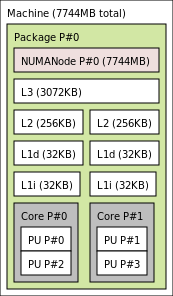
\includegraphics[width=0.25\textwidth]{Figures/ideapad-topo.png}
	\linebreak
	\caption{Η τοπολογία ενός Intel\textsuperscript{\textregistered} Core\textsuperscript{\texttrademark} i3-7100U.}
	\label{fig:ideapad-topo}
\end{figure}


\section{Συστήματα NUMA}
\label{sec:NUMA Systems}
Στην Υποενότητα \ref{ssec:Classification based on memory organization} περιγράφηκε η οργάνωση των συστημάτων ανομοιόμορφης προσπέλασης μνήμης (NUMA), τα οποία αποτελούν αρχιτεκτονική εξέλιξη των Συμμετρικών Πολυεπεξεργαστών (SMPs) που επιτρέπει την κατασκευή μεγαλύτερων παράλληλων συστημάτων.

Η πιο συχνή υλοποίηση των συστημάτων NUMA είναι ως ένα σύνολο κόμβων τύπου SMP που διαθέτουν ιεραρχία κρυφών μνημών συνδεδεμένους μεταξύ τους με ένα δίκτυο διασύνδεσης \cite{dobson2003linux}. Το δίκτυο διασύνδεσης μπορεί να είναι δακτύλιος (ring), διακοπτικό δίκτυο τύπου crossbar, από σημείο σε σημείο (point-to-point) ή πλέγμα (mesh).

Η εξασφάλιση της συνοχής των κρυφών μνημών συνήθως επιτυγχάνεται με τη χρήση ενός πρωτοκόλλου εντός του κόμβου και ενός δεύτερου πρωτοκόλλου μεταξύ των κόμβων. Όπως αναφέρθηκε νωρίτερα, ένας κόμβος SMP βασίζεται σε δίαυλο, ενώ η επικοινωνία μεταξύ των κόμβων γίνεται με πιο πολύπλοκα δίκτυα διασύνδεσης. Για το λόγο αυτό, το πρωτόκολλο συνοχής εντός του κόμβου είναι τύπου παρακολούθησης (snooping protocol), ενώ αυτό μεταξύ των κόμβων βασίζεται σε καταλόγους (directory-based protocol). Φυσικά, σε διαφορετικές οργανώσεις συστημάτων NUMA μπορούμε να συναντήσουμε και άλλες στρατηγικές επίτευξης συνοχής, όπως αυτή της μη αποθήκευσης κοινόχρηστων δεδομένων στις κρυφές μνήμες.

Όπως γίνεται γρήγορα αντιληπτό, ο προγραμματισμός αυτών των συστημάτων συνήθως απαιτεί να εστιάσουμε στην τοπικότητα, δηλαδή τη χρήση πόρων που βρίσκονται στη μικρότερη δυνατή απόσταση και την μείωση της επικοινωνίας μεταξύ των κόμβων \cite{bligh2004linux}. Για την επίτευξη της τοπικότητας και άρα τη συγγραφή πιο αποδοτικών προγραμμάτων, η εκμετάλλευση πληροφορίας που σχετίζεται με την τοπολογία είναι απαραίτητη.

Στο Σχήμα \ref{fig:parade-topo} φαίνεται η οργάνωση του \texttt{parade}, ενός NUMA συστήματος με τέσσερις κόμβους τύπου SMP που διαθέτει η Ομάδα Παράλληλης Επεξεργασίας του Πανεπιστημίου Ιωαννίνων και η οργάνωσή του αποτελεί την πλέον συνηθισμένη.

\begin{figure}[t]
	\centering
	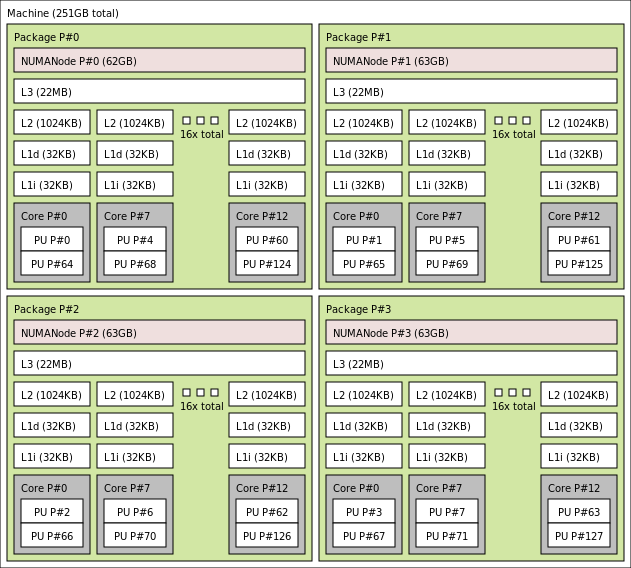
\includegraphics[width=0.8\textwidth]{Figures/parade-topo.png}
	\linebreak
	\caption{Η τοπολογία ενός Dell PowerEdge R840 με 4 Intel\textsuperscript{\textregistered} Xeon\textsuperscript{\textregistered} Gold 6130.}
	\label{fig:parade-topo}
\end{figure}


\section{Βοηθητικά Εργαλεία}
\label{sec:Utility Tools}
Για την εκμετάλλευση της τοπολογίας ενός συστήματος έχουν αναπτυχθεί διάφορα εργαλεία όπως η βιβλιοθήκη Portable Hardware Locality (hwloc) και η \texttt{libnuma}.

\subsection{hwloc}
\label{ssec:hwloc}
Η βιβλιοθήκη Portable Hardware Locality παρέχει μία φορητή αφαίρεση (abstraction) της τοπολογίας που διαθέτουν υπολογιστικά συστήματα με σύγχρονες αρχιτεκτονικές. Ο κύριος λόγος χρήσης της είναι η συγκέντρωση πληροφοριών σχετικά με πολύπλοκα παράλληλα συστήματα, με στόχο την κατάλληλη και αποδοτική εκμετάλλευσή τους \cite{broquedis2010hwloc}. 

\noindent Τα λειτουργικά συστήματα που υποστηρίζονται είναι τα εξής:
\begin{itemize}
	\item Linux
	\item Solaris, AIX, HP-UX
	\item NetBSD, FreeBSD, kFreeBSD/GNU
	\item Darwin / OS X
	\item Microsoft Windows
	\item IBM BlueGene/Q Compute Node Kernel (CNK)
\end{itemize}

\subsubsection{Τα στοιχεία που απαρτίζουν την τοπολογία}
Η hwloc μπορεί να αναγνωρίσει τα εξής στοιχεία υλικού:
\begin{itemize}
	\item Κόμβους συστημάτων NUMA (NUMA nodes)
	\item Υποδοχές επεξεργαστών (packages, πρώην sockets)
	\item Κρυφές μνήμες (caches)
	\item Πυρήνες (cores)
	\item H/W threads (PUs - Processing Units)
	\item Σύσκευές εισόδου-εξόδου όπως:
	\begin{itemize}
		\item Συσκευές PCI
		\item Επιταχυντές OpenCL, CUDA και Xeon Phi
		\item Προσαρμογείς δικτύου (network interfaces) όπως InfiniBand	
	\end{itemize}
\end{itemize}

Με την ορολογία της hwloc στη διάθεση μας, ας ανατρέξουμε στο Σχήμα \ref{fig:parade-topo} που απεικονίζεται η τοπολογία του συστήματος parade. Στο σχήμα αυτό βλέπουμε 4 επεξεργαστές ο καθένας εκ των οποίων διαθέτει 12 πυρήνες, και ιεραρχία κρυφών μνημών τριών επιπέδων (L1i \& L1d, L2, L3). Τα επίπεδα ένα και δύο των κρυφών μνημών είναι κοινά ανά πυρήνα, ενώ το επίπεδο τρία είναι κοινό για όλους τους πυρήνες του επεξεργαστή. Επίσης, κάθε πυρήνας διαθέτει δύο H/W threads τα οποία μοιράζονται τους πόρους του πυρήνα (π.χ. κρυφές μνήμες).

\subsubsection{Οι εντολές lstopo και lstopo-no-graphics}
Οι εντολές \texttt{lstopo} και \texttt{lstopo-no-graphics} συμπεριλαμβάνονται στην hwloc και χρησιμοποιούνται για την προβολή της τοπολογίας ενός συστήματος σε διαφορετικές μορφές, όπως κείμενο ASCII, SVG, PDF, Postscript, PNG, XML και αρκετές άλλες.

Τα Σχήματα \ref{fig:ideapad-topo} και \ref{fig:parade-topo} είναι αποτέλεσμα αυτών των δύο εντολών. Η αναπαράσταση του Σχήματος \ref{fig:ideapad-topo} σε μορφή κειμένου ASCII είναι η ακόλουθη\footnote{Για λόγους απλότητας έχουν παραλειφθεί οι συσκευές Εισόδου/Εξόδου και από τις δύο αναπαραστάσεις.}:

\begin{verbatim}
Machine (7744MB total)
  Package L#0
    NUMANode L#0 (P#0 7744MB)
    L3 L#0 (3072KB)
      L2 L#0 (256KB) + L1d L#0 (32KB) + L1i L#0 (32KB) + Core L#0
        PU L#0 (P#0)
        PU L#1 (P#2)
      L2 L#1 (256KB) + L1d L#1 (32KB) + L1i L#1 (32KB) + Core L#1
        PU L#2 (P#1)
        PU L#3 (P#3)
\end{verbatim}

Η διαφορά των δύο εντολών είναι ότι η δυνατότητα γραφικής αναπαράστασης (π.χ. PNG) υπάρχει μόνο στην πρώτη. Αυτό συμβαίνει για τη μείωση των εξαρτήσεων με τις σχετικές βιβλιοθήκες γραφικών που χρησιμοποιούνται για τη δημιουργία των οπτικοποιήσεων. Για παράδειγμα, στο σύστημα parade που χρησιμοποιείται για τη διεξαγωγή πειραματικών μετρήσεων δεν υπάρχουν οι απαραίτητες βιβλιοθήκες γραφικών. Για το λόγο αυτό χρησιμοποιήθηκε η εντολή \texttt{lstopo-no-graphics} για την αποθήκευση της τοπολογίας σε μορφή XML και σε διαφορετικό σύστημα με τις κατάλληλες βιβλιοθήκες εγκατεστημένες χρησιμοποιήθηκε η μορφή XML ως είσοδος στην εντολή \texttt{lstopo} για την παραγωγή αρχείου PNG.


\subsubsection{Η διεπαφή προγραμματισμού εφαρμογών (API)}
Η βασική διεπαφή προγραμματισμού εφαρμογών (API) της hwloc είναι διαθέσιμη μέσω του αρχείου \texttt{hwloc.h}, ενώ για την επιτυχή μετάφραση χρειάζεται το όρισμα \texttt{-lhwloc}.

Η τοπολογία του υποκείμενου συστήματος αναπαρίσταται ως μία δεντρική δομή από αντικείμενα και αποθηκεύεται σε μία μεταβλητή τύπου \texttt{hwloc\_topology\_t}. Στη ρίζα του δέντρου υπάρχει πάντα ένα αντικείμενο τύπου Machine που αναπαριστά ολόκληρο το υποκείμενο μηχάνημα/σύστημα, ενώ στα φύλλα του δέντρου υπάρχουν πάντα PUs ή αλλιώς H/W threads που αποτελούν το μικρότερο διαθέσιμο επεξεργαστικό στοιχείο. Καμία άλλη παραδοχή δεν είναι δυνατόν να γίνει για τη μορφή της τοπολογίας (π.χ. βάθος, τύποι αντικειμένων που την απαρτίζουν κλπ).

Για τη διαχείριση της μεταβλητής τύπου \texttt{hwloc\_topology\_t} χρησιμοποιούνται οι εξής βασικές συναρτήσεις των οποίων η λειτουργία είναι εύκολα κατανοητή από το όνομά τους:
\begin{itemize}
	\item \texttt{hwloc\_topology\_init()}
	\item \texttt{hwloc\_topology\_load()}
	\item \texttt{hwloc\_topology\_destroy()}
\end{itemize}

Αφού αρχικοποιηθεί και φορτωθεί η τοπολογία με τις δύο πρώτες κλήσεις, μπορεί να γίνει αναδρομική διάσχιση του δέντρου για την ανακάλυψη των διαφορετικών συστατικών του στοιχείων (packages, NUMA nodes, caches, cores, PUs). Η hwloc διαθέτει πλήθος χρήσιμων συναρτήσεων που διευκολύνουν είτε την αναδρομική διάσχιση, είτε τη διάσχιση ενός μόνο επιπέδου και επιτρέπουν:
\begin{itemize}
	\item την εύρεση του αντικειμένου στη ρίζα της τοπολογίας (\texttt{hwloc\_get\_root\_obj()}).
	\item την εύρεση του πλήθους των αντικειμένων που έχουν συγκεκριμένο τύπο ή βάθος (\texttt{hwloc\_get\_nbobjs\_by\_type()} και \texttt{hwloc\_get\_nbobjs\_by\_depth()}).
	\item την εύρεση αντικειμένων με συγκεκριμένο τύπο ή σε συγκεκριμένο βάθος (\texttt{hwloc\_get\_obj\_by\_type()} και \texttt{hwloc\_get\_obj\_by\_depth()}).
	\item την εύρεση του επόμενου στη σειρά αντικειμένου με συγκεκριμένο τύπο ή βάθος (\texttt{hwloc\_get\_next\_obj\_by\_type()} και \texttt{hwloc\_get\_next\_obj\_by\_depth()}).
\end{itemize}


\subsubsection{Άλλες δυνατότητες της hwloc}
Πέρα από τη συγκέντρωση πληροφοριών που σχετίζονται με την τοπολογία του υποκείμενου συστήματος, η hwloc μπορεί να χρησιμοποιηθεί για την ανάθεση νημάτων (thread binding) σε επεξεργαστές και τη διαχείριση μνήμης με δυνατότητα δέσμευσης τμημάτων μνήμης σε συγκεκριμένους κόμβους NUMA (memory binding). Παρόλα αυτά, η χρήση των διαθέσιμων λειτουργιών υπόκειται στις δυνατότητες του εκάστοτε λειτουργικού συστήματος.


\subsection{libnuma}
Η libnuma είναι μία βιβλιοθήκη που παρέχει μία διεπαφή προγραμματισμού εφαρμογών (API) για την πολιτική NUMA (NUMA policy) του Linux Kernel.

Η πολιτική NUMA του Linux αφορά τη δέμευση μνήμης σε συγκεκριμένους κόμβους NUMA ώστε να μπορεί το πρόγραμμα που εκτελείται να την προσβεί όσο το δυνατόν πιο γρήγορα \cite{kleen2005numa}. Η προκαθορισμένη πολιτική του Linux είναι η δέσμευση μνήμης να πραγματοποιείται στον τοπικό κόμβο του νήματος που την προκάλεσε \cite[\texttt{mm/mempolicy.c}]{linux}. Ένα νήμα προκαλεί δέσμευση μνήμης όταν γράψει για πρώτη φορά σε μία εικονική διεύθυνση\footnote{Το λειτουργικό σύστημα χρησιμοποιεί έναν μηχανισμό γνωστό ως εικονική μνήμη (virtual memory) ώστε να μπορεί να παρέχει σε κάθε διεργασία ένα συνεχόμενο χώρο (εικονικών) διευθύνσεων ικανοποιητικού μεγέθους (π.χ. 4 Gigabytes για συστήματα 32 bit), ακόμα και αν αυτός ο χώρος δεν είναι διαθέσιμος στη φυσική μνήμη (π.χ. 8 Gigabytes).} που ανήκει σε σελίδα\footnote{Η εικονική και φυσική μνήμη είναι χωρισμένες σε τμήματα, συνήθως μεγέθους 4,096 Bytes, που ονομάζονται σελίδες (pages).} (page) της εικονικής μνήμης η οποία δεν έχει αντιστοιχιστεί σε σελίδα φυσικής μνήμης. Αυτή η πολιτική είναι γνωστή και ως first-touch. 

Η πολιτική first-touch είναι αποδοτική όταν οι προσβάσεις πραγματοποιούνται από νήματα που εκτελούνται στον κόμβο όπου έχει δεσμευτεί η μνήμη. Υπάρχουν όμως περιπτώσεις που μπορεί να οδηγηθούμε σε κακές επιδόσεις. Μία τέτοια περίπτωση είναι όταν μία πολυνηματική εφαρμογή εκτελείται σε πολλαπλούς κόμβους αλλά μόνο ένα νήμα κάνει τις αρχικοποιήσεις της μνήμης. Κάτι τέτοιο θα οδηγήσει στη δέσμευση της μνήμης μόνο σε ένα κόμβο και άρα τα νήματα που είναι τοποθετημένα στους υπόλοιπους κόμβους θα αναγκαστούν να πραγματοποιούν απομακρυσμένες προσβάσεις με αποτέλεσμα να παρατηρηθούν αυξημένες καθυστερήσεις. Τη λύση σε αυτό το πρόβλημα μπορεί να δώσει η libnuma, καθώς επιτρέπει στο νήμα που κάνει όλες τις αρχικοποιήσεις να να δεσμεύσει μνήμη σε οποιοδήποτε κόμβο και συνεπώς να κατανείμει τη μνήμη λαμβάνοντας υπόψην από ποιό κόμβο πρόκειται να προέλθουν οι περισσότερες προσπελάσεις.

Η προκαθορισμένη πολιτική μπορεί να αλλάξει για συγκεκριμένα τμήματα μνήμης ή σε επίπεδο νήματος/διεργασίας. Στην πρώτη περίπτωση η πολιτική είναι ίδια για όλα τα νήματα/διεργασίες. Στη δεύτερη περίπτωση, η αλλαγή επηρεάζει μόνο το τρέχον νήμα/διεργασία και η νέα πολτική κληρονομείται σε νήματα/διεργασίες-παιδιά που ίσως δημιουργηθούν μεταγενέστερα. Οι διαθέσιμες πολιτικές είναι οι εξής:
\begin{itemize}
	\item page interleaving: Οι σελίδες δεσμεύονται κυκλικά (round-robin) σε όλους τους διαθέσιμους κόμβους (ή ένα υποσύνολό τους).
	\item preferred node allocation: Οι σελίδες δεσμεύονται στον επιθυμητό κόμβο.
	\item local allocation: Οι σελίδες δεσμεύονται στον τοπικό κόμβο όπου εκτελείται η διεργασία ή το νήμα.
	\item allocation only on specific nodes: Οι σελίδες δεσμεύονται μόνο σε συγκεκριμένους κόμβους.
\end{itemize}

Είναι σημαντικό να διευκρινιστεί ότι η διαχείριση μνήμης στη libnuma γίνεται σε επίπεδο σελίδων. Για παράδειγμα, όταν ο χρήστης αιτείται δέσμευση μνήμης συγκεκριμένου μεγέθους, αυτό το μέγεθος στρογγυλοποιείται προς τα πάνω ώστε να είναι πολλαπλάσιο του μεγέθους σελίδας (page size, συνήθως 4,096 Bytes). Επίσης, η ανομοιόμορφη προσπέλαση μνήμης που προκύπτει λόγω της ύπαρξης ιεραρχίας κρυφών μνημών αγνοείται κατά τη διαδικασία ορισμού των κόμβων NUMA \cite{numaman}.

\subsubsection{Η διεπαφή προγραμματισμού εφαρμογών (API)}
Η βασική διεπαφή προγραμματισμού εφαρμογών (API) της libnuma είναι διαθέσιμη μέσω του αρχείου \texttt{numa.h}, ενώ για την επιτυχή μετάφραση χρειάζεται το όρισμα \texttt{-lnuma}.

Πριν οποιαδήποτε κλήση συνάρτησης που παρέχει η libnuma, είναι υποχρεωτικό να κληθεί η συνάρτηση \texttt{numa\_available()} και σε περίπτωση που επιστραφεί η τιμή -1 οι συναρτήσεις της libnuma είναι απροσδιόριστες (undefined).

Οι ακόλουθες συναρτήσεις δεσμεύουν μνήμη χρησιμοποιώντας κάποια από τις διαθέσιμες πολιτικές, χωρίς όμως να αλλάξουν την προκαθορισμένη πολιτική:
\begin{itemize}
	\item \texttt{numa\_alloc\_onnode()}: Δεσμεύει μνήμη σε συγκεκριμένο κόμβο.
	\item \texttt{numa\_alloc\_local()}: Δεσμεύει μνήμη στον τοπικό κόμβο.
	\item \texttt{numa\_alloc\_interleaved()} και \texttt{numa\_alloc\_interleaved\_subset()}: Δεσμεύουν \newline μνήμη κυκλικά σε όλους τους κόμβους ή σε ένα υποσύνολό τους αντίστοιχα.
	\item \texttt{numa\_alloc()}: Δεσμεύει μνήμη βάσει της τρέχουσας πολιτικής.
\end{itemize}
Η απελευθέρωση της μνήμης που δεσμεύτηκε με τις παραπάνω συναρτήσεις γίνεται μέσω της συνάρτησης \texttt{numa\_free()}, ενώ η συνάρτηση \texttt{numa\_realloc()} επιτρέπει την αλλαγή του μεγέθους της ήδη δεσμευμένης μνήμης.

Συναρτήσεις αλλαγής της προκαθορισμένης πολιτικής του τρέχοντος νήματος ή διεργασίας:
\begin{itemize}
	\item \texttt{numa\_set\_localalloc()}: Αλλάζει την πολιτική σε local allocation.
	\item \texttt{numa\_set\_preferred()}: Αλλάζει την πολιτική σε preferred node allocation και θέτει ως προτιμητέο κόμβο αυτόν που περνιέται ως παράμετρος.
	\item \texttt{numa\_set\_interleave\_mask()}: Αλλάζει την πολιτική σε page interleaving και η δέσμευση πραγματοποιείται κυκλικά στους κόμβους που καθορίζονται μέσω της μάσκας που περνιέται ως παράμετρος.
	\item \texttt{numa\_set\_membind()}: Αλλάζει την πολιτική ώστε η δέσμευση μνήμης να πραγματοποιείται μόνο από τους κόμβους που καθορίζονται μέσω της μάσκας που περνιέται ως παράμετρος.
\end{itemize}

\noindent Άλλες χρήσιμες συναρτήσεις:
\begin{itemize}
	\item \texttt{numa\_max\_node()}: Επιστρέφει το μέγιστο αναγνωριστικό κόμβου που είναι διαθέσιμο στο υποκείμενο σύστημα. 
	\item \texttt{numa\_num\_configured\_nodes()}: Επιστρέφει το πλήθος των κόμβων του υποκείμενου συστήματος συμπεριλαμβανομένων και των απενεργοποιημένων (disabled) κόμβων.
	\item \texttt{numa\_get\_mems\_allowed()}: Επιστρέφει μία μάσκα που αναπαριστά τους κόμβους στους οποίους  η τρέχουσα διεργασία μπορεί να δεσμεύσει μνήμη.
	\item \texttt{numa\_num\_configured\_cpus()}: Επιστρέφει το πλήθος των επεξεργαστών του υποκείμενου συστήματος συμπεριλαμβανομένων και όσων είναι απενεργοποιημένοι (disabled).
	\item \texttt{numa\_node\_size()}: Επιστρέφει το μέγεθος της μνήμης ενός κόμβου και προεραιτικά (μέσω παραμέτρου) το μέγεθος της διαθέσιμης προς δέσμευση μνήμης.
	\item \texttt{numa\_pagesize()}: Επιστρέφει το μέγεθος της σελίδας σε bytes.
	\item \texttt{numa\_node\_of\_cpu()}: Επιστρέφει το αναγνωριστικό του κόμβου στον οποίο ανήκει ένας επεξεργαστής\footnote{Ότιδήποτε ορίζει το λειτουργικό σύστημα ως επεξεργαστή. Στην περίπτωση του Linux Kernel, οποιοδήποτε επεξεργαστικό στοιχείο που μπορεί να εκτελέσει μία διεργασία, όπως για παράδειγμα ένα H/W thread.}.
\end{itemize}


\subsubsection{Άλλες δυνατότητες της libnuma}
Η libnuma υποστηρίζει μεταξύ άλλων, λειτουργίες όπως η αλλαγή της πολιτικής ήδη δεσμευμένης μνήμης, περιορισμού της εκτέλεσης ενός νήματος/διεργασίας σε συγκεκριμένο σύνολο κόμβων ή επεξεργαστών, εύρεσης της απόστασης μεταξύ δύο κόμβων, μετακίνησης σελίδων μεταξύ κόμβων, καθώς και πληθώρα συναρτήσεων διαχείρισης μασκών που χρησιμοποιούνται για την αναπαράσταση συνόλων από κόμβους ή επεξεργαστές.

% \subsubsection{Οι εντολές numactl και numastat}

% Ήδη από την έκδοση 2.5 του Linux Kernel προστέθηκε η βασική υποδομή για υποστήριξη συστημάτων NUMA, που περιλαμβάνει μεταξύ άλλων αναγνώριση της τοπολογίας, δέσμευση μνήμης και χρονοδρομολόγηση διεργασιών.

\newpage

\section{Χρήση τοπολογίας στο OpenMP}
\label{sec:Topology in OpenMP}
Στην έκδοση 4.0 του OpenMP προστέθηκε η δυνατότητα ανάθεσης (binding) των νημάτων σε σύνολα από συγκεκριμένους επεξεργαστές, τα λεγόμενα OpenMP places. Η ανάθεση αυτή γίνεται βάσει των διάφορων διαθέσιμων πολιτικών που περιγράφονται στις προδιαγραφές του OpenMP και είναι γνωστές ως processor binding policies. Με αυτό τον τρόπο το OpenMP δίνει τη δυνατότητα εκμετάλλευσης της τοπολογίας του υποκείμενου συστήματος ώστε, για τους λόγους που αναφέραμε στην αρχή του κεφαλαίου, να μπορούν να συγγραφούν πιο αποδοτικά παράλληλα προγράμματα.

Σε αυτό το σημείο χρειάζεται να διευκρινιστεί ότι επεξεργαστής (processor) είναι μία αυθαίρετη έννοια που προσδιορίζεται από την εκάστοτε υλοποίηση του OpenMP και αφορά μονάδα του υλικού στην οποία μπορούν να εκτελεστούν ένα ή περισσότερα νήματα. Τυπικά, ένας επεξεργαστής αντιστοιχεί σε ένα H/W thread.

Κατά το binding η εκτέλεση των νημάτων περιορίζεται σε ένα υποσύνολο των διαθέσιμων επεξεργαστών και μπορεί να χρησιμοποιηθεί για την επίτευξη καλύτερων επιδόσεων. Καλύτερες επιδόσεις μπορούμε να πετύχουμε, για παράδειγμα, περιορίζοντας τις μετακινήσεις των νημάτων μεταξύ διαφορετικών επεξεργαστών και άρα μειώνοντας\footnote{Υπό προϋποθέσεις, όπως για παράδειγμα, κατά τη διάρκεια διακοπής (interupt) να μην εκτελεστεί στον ίδιο επεξεργαστή άλλο νήμα που θα γεμίσει την κρυφή μνήμη με δικά του δεδομένα.} το πλήθος χρονοβόρων διαδικασιών όπως διαχείριση αστοχιών κρυφής μνήμης (cache misses). Επίσης, το binding μπορεί να χρησιμοποιηθεί σε πολύπλοκα συστήματα (π.χ. NUMA) για την καλύτερη κατανομή των νημάτων ανάλογα την παράλληλη εφαρμογή.

Υποθέτοντας ένα σύστημα NUMA, αν η παράλληλη εφαρμογή απαιτεί συνεργασία μεταξύ των νημάτων για την εκτέλεση μίας εργασίας, τότε συμφέρει τα νήματα να τοποθετηθούν κοντά\footnote{Βάσει της τοπολογίας του συστήματος.} το ένα στο άλλο ώστε να μπορούν να ανταλλάσσουν πιο γρήγορα δεδομένα μέσω της κρυφής και τοπικής μνήμης. Αν τα νήματα τοποθετηθούν σε διαφορετικούς κόμβους NUMA, το επικοινωνιακό φορτίο στο δίκτυο διασύνδεσης θα είναι αυξημένο λόγω του συντονισμού, συγχρονισμού και της μεταξύ τους επικοινωνίας, καθώς και λόγω της κίνησης πο δημιουργεί το πρωτοκόλλο συνοχής των κρυφών μνημών. Σε αντίθετη περίπτωση, αν οι εργασίες που ανατίθενται στα νήματα είναι ανεξάρτητες μεταξύ τους, τότε βολεύει η διασπορά των νημάτων στους κόμβους ώστε να μπορεί το κάθε νήμα να εκμεταλλευτεί τους πόρους ολόκληρου κόμβου.


\subsection{OpenMP Places}
Όπως αναφέρθηκε ήδη, τα OpenMP places, στα οποία από εδώ και στο εξής θα αναφερόμαστε απλά ως places, είναι σύνολα επεξεργαστών τα οποία χρησιμοποιούνται για την ανάθεση των νημάτων OpenMP σε αυτά βάσει των processor binding policies.

Κάθε place είναι ένα υποσύνολο των διαθέσιμων επεξεργαστών του υποκείμενου συστήματος και κάθε επεξεργαστής αναπαρίσταται μέσω ενός μοναδικού μη αρνητικού ακέραιου αριθμητικού αναγνωριστικού, η σημασία του οποίου καθορίζεται από την εκάστοτε υλοποίηση του OpenMP.

Όλα τα places μαζί αποτελούν το αρχικό place partition, το οποίο είναι η λίστα με τα places που είναι διαθέσιμα στο σύστημα χρόνου εκτέλεσης του OpenMP. Κάθε νήμα διαθέτει δικό του αντίγραφο του place partition και το οποίο ανάλογα την πολιτική ανάθεσης των νημάτων σε επεξεργαστές, μπορεί να είναι υποσύνολο του αρχικού place partition. Με τις πολιτικές ανάθεσης θα ασχοληθούμε στην Υποενότητα \ref{ssec:Processor binding policies}.

Η μεταβλητή περιβάλλοντος \texttt{OMP\_PLACES} χρησιμοποιείται για την αρχικοποίηση του αρχικού place partition. Οι έγκυρες τιμές της \texttt{OMP\_PLACES} μπορεί να έχουν δύο μορφές:
\begin{itemize}
	\item Αφηρημένο όνομα (abstract name): Περιγράφει με αφηρημένο τρόπο ένα σύνολο places (π.χ. \texttt{cores}).
	\item Ρητή λίστα (explicit list): Περιγράφει κάθε place με ρητό τρόπο χρησιμοποιώντας μη αρνητικούς ακέραιους αριθμούς.
\end{itemize}

Η ρητή λίστα, μπορεί να οριστεί ως ένα σύνολο ενός ή περισσότερων places χωρισμένων μεταξύ τους με κόμμα. Κάθε place μπορεί να περιγραφεί είτε ως ένας αριθμός, είτε ως ένα σύνολο αριθμών που περικλείονται από άγκιστρα.

Για τον ορισμό των places μπορούν επίσης να χρησιμοποιηθούν διαστήματα (intervals) μέσω του συμβολισμού \texttt{<lower-bound>:<length>:<stride>} για να περιγράψουν την εξής ακολουθία αριθμών:
\begin{itemize}
	\item \texttt{<lower-bound>}
	\item \texttt{<lower-bound>} + \texttt{<stride>}
	\item ...
	\item \texttt{<lower-bound>} + (\texttt{<length>} -1) * \texttt{<stride>}
\end{itemize}
Αν η τιμή του \texttt{<stride>} παραλείπεται, τότε θεωρείται ίση με τη μονάδα. Τα διαστήματα μπορούν να χρησιμοποιηθούν και για την περιγραφή ακολουθιών από places.

Ο τελεστής "\texttt{!}" μπορεί να χρησιμοποιηθεί για την εξαίρεση του αριθμού/place που ακολουθεί αμέσως μετά.

\noindent Εναλλακτικά, τα ακόλουθα αφηρημένα ονόματα μπορούν να χρησιμοποιηθούν για την περιγραφή των places:
\begin{itemize}
	\item \texttt{threads}: Κάθε place αντιστοιχεί σε ένα H/W thread.
	\item \texttt{cores}: Κάθε place αντιστοιχεί σε έναν πυρήνα αποτελούμενος από ένα ή περισσότερα H/W threads.
	\item \texttt{ll\_caches}: Κάθε place αντιστοιχεί σε ένα σύνολο πυρήνων που μοιράζονται το τελευταίο επίπεδο κρυφής μνήμης.
	\item \texttt{numa\_domains}: Κάθε place αντιστοιχεί σε ένα σύνολο πυρήνων των οποίων η πιο κοντινή μνήμη σε αυτούς:
	\begin{itemize}
		\item είναι η ίδια μνήμη και % TODO verify!!!
		\item σε παρόμοια απόσταση από τους πυρήνες.
	\end{itemize}
	\item \texttt{sockets}: Κάθε place αντιστοιχεί σε μία υποδοχή ολοκληρωμένου κυκλώματος επεξεργαστή (socket).
\end{itemize}

Τα αφηρημένα ονόματα μπορούν να ακολουθούνται από ένα ακέραιο νούμερο μέσα σε παρενθέσεις για τον προσδιορισμό του πλήθους των places που θα αποτελέσουν το αρχικό place partition (π.χ. \texttt{threads(8)}). Σε περίπτωση που ζητηθούν λιγότερα places σε σχέση με τα διαθέσιμα, η υλοποίηση του OpenMP αποφασίζει ποιά places θα περιληφθούν στο place partition. Αν ζητηθούν περισσότερα places, η υλοποίηση του OpenMP καθορίζει το μέγεθος του place partition, δηλαδή το πλήθος των places που το απαρτίζουν.

Η υλοποίηση του OpenMP καθορίζει την ακριβή σημασία των αφηρημένων ονομάτων, μπορεί να ορίσει και επιπλέον ονόματα.

Οι παρακάτω εντολές \texttt{export}\footnote{Σύνταξη συμβατή με το Bourne Again SHell (BASH).} αναθέτουν τιμή στη μεταβλητή \texttt{OMP\_PLACES}, ορίζοντας και οι πέντε ακριβώς τα ίδια τέσσερα places:
\begin{itemize}
	\item \texttt{export OMP\_PLACES=threads}
	\item \texttt{export OMP\_PLACES="threads(4)"}
	\item \texttt{export OMP\_PLACES="{0,1,2,3},{4,5,6,7},{8,9,10,11},{12,13,14,15}"}
	\item \texttt{export OMP\_PLACES="{0:4},{4:4},{8:4},{12:4}"}
	\item \texttt{export OMP\_PLACES="{0:4}:4:4"}
\end{itemize}


\subsubsection{Η σύνταξη της μεταβλητής περιβάλλοντος OMP\_PLACES}
\label{ssec:OMP Places syntax}
Το σύνολο των έγκυρων τιμών που μπορούν να ανατεθούν στη μεταβλητή \texttt{OMP\_PLACES} σύμφωνα με το OpenMP 5.1 \cite{openmp51} προκύπτουν βάσει των ακόλουθων συντακτικών κανόνων:
\begin{verbatim}
	<list>         |= <p-list> | <aname>
	<p-list>       |= <p-interval> | <p-list>,<p-interval>
	<p-interval>   |= <place>:<len>:<stride> | <place>:<len> | <place> | !<place>
	<place>        |= {<res-list>} | <res>
	<res-list>     |= <res-interval> | <res-list>,<res-interval>
	<res-interval> |= <res>:<num-places>:<stride> | <res>:<num-places> | <res>
	                  | !<res>
	<aname>        |= <word>(<num-places>) | <word>
	<word>         |= sockets | cores | ll_caches | numa_domains | threads
	                  | <implementation-defined abstract name>
	<res>          |= non-negative integer
	<num-places>   |= positive integer
	<stride>       |= integer
	<len>          |= positive integer
\end{verbatim}


\subsection{OpenMP Processor Binding Policies}
\label{ssec:Processor binding policies}

%Ο χρήστης έχει τη δυνατότητα προσδιορισμού της λίστας των διαθέσιμων OpenMP places αλλά και της πολιτικής ανάθεσης των νημάτων σε αυτά.

% για την εξισορρόπηση του φορτίου\footnote{Αν υποθέσουμε ότι η εργασία μπορεί να ισοκατανεμηθεί και ότι το υποκείμενο σύστημα είναι αφοσιωμένο (dedicated) στην εκτέλεση της παράλληλης εφαρμογής.} (load balancing),